\documentclass{standalone}
\usepackage{pgfplots}
\pgfplotsset{compat=newest}
\usetikzlibrary{decorations.markings}
\tikzset{->-/.style={decoration={
  markings,
  mark=at position #1 with {\arrow{>}}},postaction={decorate}}}
  \tikzset{-<-/.style={decoration={
  markings,
  mark=at position #1 with {\arrow{<}}},postaction={decorate}}}
\begin{document}
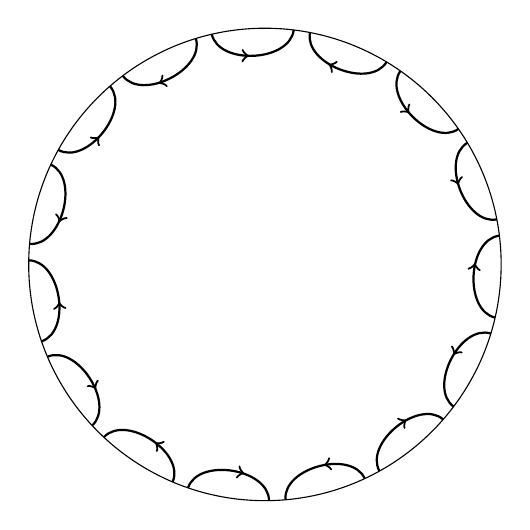
\begin{tikzpicture}[scale=2]

% \path (180:1.5) coordinate (a);
% \path (0:1.5) coordinate (b);
% \foreach \phi in {-30,0,...,30}{
%   \draw[dashed] (a) to[out={\phi},in={180-\phi}] (b);
% }
% \foreach \phi in {60,-60}{
%   \draw[dashed] (a) .. controls ++(\phi:1.5) and ++({180-\phi}:1.5) .. (b);
% }
% \draw[draw=none, fill=white] (a) circle (0.32cm);
% \draw[draw=none, fill=white] (b) circle (0.32cm);

\draw (0,0) circle (1.5cm);

% \foreach \r in {0.2,0.3,...,1.5}{
%   \draw[dashed,-<-=0.5] (0,0) circle (\r cm);
% }

\foreach \rot in {0,48,...,360}{
  \begin{scope}[rotate=\rot]
  \path (55:1.5) coordinate (A);
  \path  ({45+(45-55)}:1.5) coordinate (B);
  \draw[->-=0.45,thick] (A) to[out={55-180},in=-{55-90}] (B);
  \end{scope}
}

\foreach \rot in {24,72,...,320}{
  \begin{scope}[rotate=\rot]
  \path (55:1.5) coordinate (A);
  \path  ({45+(45-55)}:1.5) coordinate (B);
  \draw[-<-=0.45,thick] (A) to[out={55-180},in=-{55-90}] (B);
  \end{scope}
}

% \begin{scope}[rotate=90]
% \foreach \phi in {10,20,30}{
%   \path (\phi:1.5) coordinate (A);
%   \path  ({45+(45-\phi)}:1.5) coordinate (B);
%   \draw[-<-=0.45,thick] (A) to[out={\phi-180},in=-{\phi-90}] (B);
% }  
% \end{scope}

% \begin{scope}[rotate=180]
% \foreach \phi in {10,20,30}{
%   \path (\phi:1.5) coordinate (A);
%   \path  ({45+(45-\phi)}:1.5) coordinate (B);
%   \draw[->-=0.45,thick] (A) to[out={\phi-180},in=-{\phi-90}] (B);
% }  
% \end{scope}

% \begin{scope}[rotate=-90]
% \foreach \phi in {10,20,30}{
%   \path (\phi:1.5) coordinate (A);
%   \path  ({45+(45-\phi)}:1.5) coordinate (B);
%   \draw[-<-=0.45,thick] (A) to[out={\phi-180},in=-{\phi-90}] (B);
% }  
% \end{scope}
% \foreach \phi in {18,162}{
%   \path (\phi:1.5) coordinate (A);
%   \path  ({180+(180-\phi)}:1.5) coordinate (B);
%   % \draw  to[, in=0];
%   \draw[draw=none,fill=white] (A) to[out={\phi-180},in=-{\phi-180}] (B) -- cycle;
% }

% \draw[-<-=0.5,thick] (0,0) -- (180:1.5);
% \draw[-<-=0.5,thick] (0,0) -- (0:1.5);
% \draw[->-=0.5,thick] (0,0) -- (90:1.5);
% \draw[->-=0.5,thick] (0,0) -- (-90:1.5);

\end{tikzpicture}
\end{document}
